\documentclass{article}

%%%%%%%%%%%%%%%%%%%%%%%%%%%%%%%%%%%%%%%%%
% Lachaise Assignment
% Structure Specification File
% Version 1.0 (26/6/2018)
%
% This template originates from:
% http://www.LaTeXTemplates.com
%
% Authors:
% Marion Lachaise & François Févotte
% Vel (vel@LaTeXTemplates.com)
%
% License:
% CC BY-NC-SA 3.0 (http://creativecommons.org/licenses/by-nc-sa/3.0/)
% 
%%%%%%%%%%%%%%%%%%%%%%%%%%%%%%%%%%%%%%%%%

%----------------------------------------------------------------------------------------
%	PACKAGES AND OTHER DOCUMENT CONFIGURATIONS
%----------------------------------------------------------------------------------------

\usepackage{amsmath,amsfonts,stmaryrd,amssymb} % Math packages

\usepackage[ddmmyyyy]{datetime}
\usepackage{enumerate} % Custom item numbers for enumerations

\usepackage[ruled]{algorithm2e} % Algorithms

\usepackage[framemethod=tikz]{mdframed} % Allows defining custom boxed/framed environments

\usepackage{listings} % File listings, with syntax highlighting
\lstset{
  language=C,
  basicstyle=\ttfamily\small\color{black},
  numbers=left,
  numberstyle=\small\color{gray},
  stepnumber=1,
  numbersep=4pt,
  frame=single,
  rulecolor=\color{black},
  framesep=5pt,
  xleftmargin=20pt,
  framexleftmargin=15pt,
  breaklines=true,
  showstringspaces=false,
  keywordstyle=\color{purple}\bfseries,          % parole chiave (if, else, int, return...)
  commentstyle=\color{teal}\itshape,           % commenti
  stringstyle=\color{orange},                   % stringhe
  identifierstyle=\color{black},                % identificatori normali
  emph={size_t, uint32_t, uint64_t, TAS, RTE},            % tipi aggiuntivi
  emphstyle=\color{blue}\bfseries,            % stile tipi aggiuntivi
  morekeywords={uint8_t, uint16_t, uint32_t, uint64_t, int8_t, int16_t, int32_t, int64_t, bool, true, false}, % tipi e parole chiave extra
  morecomment=[l]{//},                           % commenti con //
  morecomment=[s]{/*}{*/},                       % commenti multilinea
}

\lstdefinelanguage{RISCAsm}{
  morekeywords={
    ADDQ, SUM, ANDI, MOVE,MOVEA, MOVEM, DC, DS, sra, 
    lw, sw, li, la, mv, 
    BEQ, BNE, JMP, CMP, jalr, ret, 
    NOP, lui, RTE, RTS, 
    ecall, ebreak, ORG, EQU, JSR, CLR, TAS 
  },
  sensitive=true,
  morecomment=[l]{\*},
  morestring=[b]",
  basicstyle=\ttfamily\small\color{black},
  keywordstyle=\color{purple}\bfseries,
  commentstyle=\color{teal}\itshape,
  stringstyle=\color{orange},
  numbers=left,
  numberstyle=\small\color{gray},
  stepnumber=1,
  numbersep=4pt,
  frame=single,
  rulecolor=\color{black},
  framesep=5pt,
  xleftmargin=20pt,
  framexleftmargin=15pt,
  showstringspaces=false,
  breaklines=true,
}

%----------------------------------------------------------------------------------------
%	DOCUMENT MARGINS
%----------------------------------------------------------------------------------------

\usepackage{geometry} % Required for adjusting page dimensions and margins

\geometry{
	paper=a4paper, % Paper size, change to letterpaper for US letter size
	top=2.5cm, % Top margin
	bottom=3cm, % Bottom margin
	left=2.5cm, % Left margin
	right=2.5cm, % Right margin
	headheight=14pt, % Header height
	footskip=1.5cm, % Space from the bottom margin to the baseline of the footer
	headsep=1.2cm, % Space from the top margin to the baseline of the header
	%showframe, % Uncomment to show how the type block is set on the page
}

%----------------------------------------------------------------------------------------
%	FONTS
%----------------------------------------------------------------------------------------

\usepackage[utf8]{inputenc} % Required for inputting international characters
\usepackage[T1]{fontenc} % Output font encoding for international characters

\usepackage{XCharter} % Use the XCharter fonts
\usepackage{enumitem}
\usepackage{xcolor}
\usepackage{tikz} 
\usetikzlibrary{positioning}

% pseudocode environment %


%----------------------------------------------------------------------------------------
%	COMMAND LINE ENVIRONMENT
%----------------------------------------------------------------------------------------

% Usage:
% \begin{commandline}
%	\begin{verbatim}
%		$ ls
%		
%		Applications	Desktop	...
%	\end{verbatim}
% \end{commandline}

\mdfdefinestyle{commandline}{
	leftmargin=10pt,
	rightmargin=10pt,
	innerleftmargin=15pt,
	middlelinecolor=black!50!white,
	middlelinewidth=2pt,
	frametitlerule=false,
	backgroundcolor=black!5!white,
	frametitle={Command Line},
	frametitlefont={\normalfont\sffamily\color{white}\hspace{-1em}},
	frametitlebackgroundcolor=black!50!white,
	nobreak,
}

% Define a custom environment for command-line snapshots
\newenvironment{commandline}{
	\medskip
	\begin{mdframed}[style=commandline]
}{
	\end{mdframed}
	\medskip
}

%----------------------------------------------------------------------------------------
%	FILE CONTENTS ENVIRONMENT
%----------------------------------------------------------------------------------------

% Usage:
% \begin{file}[optional filename, defaults to "File"]
%	File contents, for example, with a listings environment
% \end{file}

\mdfdefinestyle{file}{
    innertopmargin=1.6\baselineskip,
    innerbottommargin=0.8\baselineskip,
    topline=false, bottomline=false,
    leftline=false, rightline=false,
    leftmargin=2cm,
    rightmargin=2cm,
    singleextra={
        \draw[fill=black!10!white](P)++(0,-1.2em)rectangle(P-|O);
        \node[anchor=north west] at(P-|O){\ttfamily\mdfilename};
        \def\l{3em}
        \draw(O-|P)++(-\l,0)--++(\l,\l)--(P)--(P-|O)--(O)--cycle;
        \draw(O-|P)++(-\l,0)--++(0,\l)--++(\l,0);
    },
}

% Comando per tab a 4 spazi all’interno dell’ambiente file
\newenvironment{file}[1][File]{%
    \medskip
    \newcommand{\mdfilename}{#1}
    % Rende il carattere tab attivo e lo definisce come 4 spazi
    \catcode`\^^I=\active
    \def^^I{\hspace*{4ex}}%
    \begin{mdframed}[style=file]
}{%
    \end{mdframed}
    \medskip
}

%----------------------------------------------------------------------------------------
%	NUMBERED QUESTIONS ENVIRONMENT
%----------------------------------------------------------------------------------------

% Usage:
% \begin{question}[optional title]
%	Question contents
% \end{question}

\mdfdefinestyle{question}{
	innertopmargin=1.2\baselineskip,
	innerbottommargin=0.8\baselineskip,
	roundcorner=5pt,
	nobreak,
	singleextra={%
		\draw(P-|O)node[xshift=1em,anchor=west,fill=white,draw,rounded corners=5pt]{%
		Question \theQuestion\questionTitle};
	},
}

\newcounter{Question} % Stores the current question number that gets iterated with each new question

% Define a custom environment for numbered questions
\newenvironment{question}[1][\unskip]{
	\bigskip
	\stepcounter{Question}
	\newcommand{\questionTitle}{~#1}
	\begin{mdframed}[style=question]
}{
	\end{mdframed}
	\medskip
}

%----------------------------------------------------------------------------------------
%	WARNING TEXT ENVIRONMENT
%----------------------------------------------------------------------------------------

% Usage:
% \begin{warn}[optional title, defaults to "Warning:"]
%	Contents
% \end{warn}

\mdfdefinestyle{warning}{
	topline=false, bottomline=false,
	leftline=false, rightline=false,
	nobreak,
	singleextra={%
		\draw(P-|O)++(-0.5em,0)node(tmp1){};
		\draw(P-|O)++(0.5em,0)node(tmp2){};
		\fill[black,rotate around={45:(P-|O)}](tmp1)rectangle(tmp2);
		\node at(P-|O){\color{white}\scriptsize\bf !};
		\draw[very thick](P-|O)++(0,-1em)--(O);%--(O-|P);
	}
}

% Define a custom environment for warning text
\newenvironment{warn}[1][Warning:]{ % Set the default warning to "Warning:"
	\medskip
	\begin{mdframed}[style=warning]
		\noindent{\textbf{#1}}
}{
	\end{mdframed}
}

%----------------------------------------------------------------------------------------
%	INFORMATION ENVIRONMENT
%----------------------------------------------------------------------------------------

% Usage:
% \begin{info}[optional title, defaults to "Info:"]
% 	contents
% 	\end{info}

\mdfdefinestyle{info}{%
	topline=false, bottomline=false,
	leftline=false, rightline=false,
	nobreak,
	singleextra={%
		\fill[black](P-|O)circle[radius=0.4em];
		\node at(P-|O){\color{white}\scriptsize\bf i};
		\draw[very thick](P-|O)++(0,-0.8em)--(O);%--(O-|P);
	}
}

% Define a custom environment for information
\newenvironment{info}[1][Info:]{ % Set the default title to "Info:"
	\medskip
	\begin{mdframed}[style=info]
		\noindent{\textbf{#1}}
}{
	\end{mdframed}
}
 % Include the file specifying the document structure and custom commands

%----------------------------------------------------------------------------------------
%	ASSIGNMENT INFORMATION
%----------------------------------------------------------------------------------------

\title{Homeworks Algorithms and Data Strucutres} % Title of the assignment

\author{Rocco Lo Russo\\ \texttt{roc.lorusso@studenti.unina.it}} % Author name and email address

\date{Università di Napoli Federico II - DIETI --- \today} % University, school and/or department name(s) and a date

%----------------------------------------------------------------------------------------

\begin{document}

\maketitle % Print the title

%----------------------------------------------------------------------------------------
%	INTRODUCTION
%----------------------------------------------------------------------------------------

\section*{Introduzione} % Unnumbered section
In questo documento verranno sviluppati i due set di Homeworks assegnati per sostenere l'esame.

\section{Homework set 1} \label{sec:homework_1}% Numbered section 
\subsection{Esercizio 1.1} \label{subsec:esercizio1_1}
\textbf{Traccia}:

\noindent
\textit{Per ognuna delle seguenti affermazioni, si dica se essa è sempre vera, mai vera, o a volte 
vera, per funzioni asintoticamente non-negative. Se la si considera sempre vera o mai vera, 
si spieghi il perché. Se è a volte vera, si dia un esempio per cui è vera e uno per cui è falsa.}
\begin{itemize}
    \item $f(n) = O(f(n)^2)$;
    \item $f(n) + O(f(n)) =  \Theta(f(n))$;
    \item $ f(n) = \Omega(g(n))$ e $f(n) = o(g(n))$
\end{itemize}
\vspace{\baselineskip}

\noindent
\textbf{Soluzione}: 

\noindent
$f(n) = O(f(n)^2) $ è un'affermazione vera a volte: infatti $f(n) = O(f(n)^2) \iff f(n) \le cf(n)^2 $ per qualche costante $ c>0 $ e per $n > n_0$. Poichè la funzione f(n) è definita asintoticamente \textit{non negativa}, possiamo assumere che per n sufficientemente grande la funzione assumerà soltanto valori o positivi o nulli. 

\noindent
Nel caso in cui $f(n) = 0$, la disuguaglianza è verificata perchè $ 0 \le c \cdot 0^2$ è vero sempre. 

\noindent
Nel caso in cui $f(n) > 0$:

\begin{equation} \label{eq:proof_1_1_1}
\begin{aligned}
f(n) &\le cf(n)^2 \implies f(n) \ge \frac{1}{c} \text{,  } \forall n \ge n_0
\end{aligned}
\end{equation}

\noindent
La disuguaglianza nel secondo caso è verificata solo se la funzione $f(n)$ risulta, per n sufficientemente grande, maggiore di $\frac{1}{c}$, ovvero se risulta limitata inferiormente da una costante strettamente maggiore di 0, come riportato nel passaggio (\ref{eq:proof_1_1_1}).
Un esempio di funzione asintoticamente non negativa che soddisfa la definizione è $f(n) = n$, mentre un esempio di funzione asintoticamente non negativa che non soddisfa la definizione è $f(n) = \frac{1}{n}$.
\vspace{\baselineskip}

\noindent
Per quanto riguarda la seconda affermazione, $f(n) + O(f(n)) =  \Theta(f(n))$, dimostriamo che è sempre vera: il generico elemento $h(n) \in \{f(n) + O(f(n))\}$ possiamo scriverlo come $h(n) = f(n) + g(n)$, con $g(n) \in O(f(n))$; I passaggi illustrati in  (\ref{eq:proof_1_1_2_1}) dimostrano che $f(n) + O(f(n)) = O(f(n))$ $\forall n \ge n_0$, mentre i passaggi illustrati in (\ref{eq:proof_1_1_2_2}) dimostrano che $f(n) + O(f(n)) = \Omega(f(n))$ $\forall n \ge n_0$. 

\begin{equation} \label{eq:proof_1_1_2_1}
\begin{aligned}
g(n) \le cf(n) \implies h(n) &= f(n) + g(n) \\ &\le f(n) + cf(n) \\ 
&\le (1+c)f(n) 
\end{aligned}
\end{equation}

\begin{equation} \label{eq:proof_1_1_2_2}
\begin{aligned}
g(n) \ge 0 \implies f(n) + g(n) \ge 1 \cdot f(n)
\end{aligned}
\end{equation}

\noindent
Possiamo concludere che il generico elemento $h(n) \in \{f(n)+O(f(n))\}$ è sia un elemento di $O(f(n))$ che un elemento di $\Omega(f(n))$, ragione per cui $\{f(n)+O(f(n))\} \subseteq {\Theta(f(n))} \implies f(n) + O(f(n)) = \Theta(f(n))$.

\vspace{\baselineskip}
\noindent
Per quanto riguarda la terza affermazione, $ f(n) = \Omega(g(n))$ e $f(n) = o(g(n))$, è sempre falsa. Intuitivamente, dire che $ f(n) = \Omega(g(n))$ significa che $f(n)$ asintoticamente cresce almeno come cresce $g(n)$, mentre dire che $f(n) = o(g(n))$ significa che $f(n)$ è asintoticamente trascurabile rispetto a $g(n)$, e questo è chiaramente in contraddizione. Verifichiamolo tramite definizioni, assumendo $f(n)$ definitivamente non negativa e $g(n)$ definitivamente positiva:

\begin{equation} \label{eq:proof_1_1_3_1}
\begin{aligned}
f(n) = \Omega(g(n)) &\implies \exists  c>0, n>n_0 \; | \; f(n) \ge cg(n) \ \forall n>n_0 \\
f(n) = o(g(n)) & \implies \lim_{n \to \infty} \frac{f(n)}{g(n)} = 0 \leftrightarrow \forall \epsilon>0 \ \exists \ n_1 \in \mathbb{N} \ \text{t.c.} \ \frac{f(n)}{g(n)} < \epsilon \ \forall \ n>n_1
\end{aligned}
\end{equation}

\noindent
Se dalla definizione del limite scegliamo $\epsilon = \frac{c}{2}$, risulta, per $n > \max\{n_0,n_1\}$, contemporaneamente $f(x) \ge cg(n)$ e $f(x) < \frac{c}{2}g(n)$, e questo è impossibile. 

\subsection{Esercizio 1.2} \label{subsec:esercizio1_2}
\textbf{Traccia}:

\noindent
\textit{Per ognuna delle seguenti coppie di funzioni $f(n)$ e $g(n)$, trovare una appropriata costante positiva c tale che $f(n) \le cg(n)$  per tutti i valori di $n > 1$.}
\begin{itemize}
    \item $f(n) = n^2 + n + 1, \quad g(n) = 2n^3$;
    \item $f(n) = n\sqrt{n} + n^2, \quad g(n) = n^2 $;
    \item $ f(n) = n^2 - n + 1, \quad g(n) = n^2/2 $
\end{itemize}
\vspace{\baselineskip}

\noindent
\textbf{Soluzione}: 

\noindent
La prima costante $c$ che soddisfi $f(n) = n^2 + n + 1 \le cg(n) = 2cn^3$ può essere facilmente trovata tramite i passaggi presentati in (\ref{eq:proof_1_2_1_1}), nei quali osserviamo che $\frac{1}{n} + \frac{1}{n^2} + \frac{1}{n^3}$ è una funzione definitivamente decrescente $\forall n>1$, e in particolare assume il valore massimo proprio in $n=1$.

\begin{equation} \label{eq:proof_1_2_1_1}
\begin{aligned}
n^2 + n + 1 \le 2cn^3 \implies \frac{n^2 + n +1}{n^3} \le 2c &\implies \frac{1}{n} + \frac{1}{n^2} + \frac{1}{n^3} \le 2c \\
3 \le 2c &\implies c \ge \frac{3}{2}
\end{aligned}
\end{equation}

\noindent
Per questo motivo, anche se stiamo assumendo $n>1$ strettamente, una costante opportuna potrebbe essere proprio $c = \frac{3}{2}$.

\vspace{\baselineskip}
\noindent
La seconda costante $c$ che soddisfi $f(n) = n\sqrt{n} + n^2 \le cg(n) = cn^2 $ può essere trovata tramite lo stesso metodo presentato sopra, ovvero osservando nei passaggi (\ref{eq:proof_1_2_2_1}) che la funzione $\frac{\sqrt{n}}{n} + 1 = \frac{1}{\sqrt{n}} + 1 $ è una funzione decrescente $\forall n > 1$, e che assume valore massimo pari a 2 proprio in $n=1$.

\begin{equation} \label{eq:proof_1_2_2_1}
\begin{aligned}
n\sqrt{n} + n^2 \le cn^2 &\implies n\sqrt{n} \le cn^2 - n^2 = n^2 (c-1) \\
&\implies c \ge \frac{1}{\sqrt{n}} + 1
\end{aligned}
\end{equation}

\noindent
Per questo motivo, anche se stiamo assumendo $n>1$, una costante opportuna potrebbe essere proprio $c = 2$.

\vspace{\baselineskip}
\noindent
La terza costante $c$ che soddisfi $ f(n) = n^2 - n + 1 \le cg(n) = cn^2/2 $ può essere trovata ancora tramite lo stesso metodo, ovvero osservando nei passaggi (\ref{eq:proof_1_2_3_1}) che la funzione $1-\frac{1}{n} + \frac{1}{n^2} $ è una funzione che per $n \rightarrow \infty $ viene limitata dal valore 1.

\begin{equation} \label{eq:proof_1_2_3_1}
\begin{aligned}
n^2 - n + 1 \le \frac{cn^2}{2} &\implies 1 - n \le \frac{cn^2}{2} - n^2 \\
&\implies 1 - n \le n^2 (\frac{c}{2} -1) \\
&\implies \frac{c}{2} \ge 1 - \frac{1}{n} + \frac{1}{n^2} \\
\end{aligned}
\end{equation}

\noindent
Per questo motivo, anche se stiamo assumendo $n>1$, una costante opportuna potrebbe essere proprio $c = 2$, e in particolare c è la costante più piccola che garantisca la diseguaglianza $\forall n>1$.

\subsection{Esercizio 1.3} \label{subsec:esercizio1_3}
\textbf{Traccia}:

\noindent
\textit{Dimostrare che per qualsiasi costante reale a e b, con b > 0, $(n+a)^b = \Theta(n^b)$}.
\vspace{\baselineskip}

\noindent
\textbf{Soluzione}: 

\begin{equation} \label{eq:proof_1_3_1_1}
\begin{aligned}
(n+a)^b = n^b\left( 1+\frac{a}{n} \right)^b
\end{aligned}
\end{equation}

\noindent
Osserviamo che se scegliamo $n_0 = 2|a|$ ad esempio, è soddisfatta la disuguaglianza $\frac{|a|}{n} < \frac{1}{2} \ \forall n>2|a|$. Possiamo continuare con la (\ref{eq:proof_1_3_1_2}): 

\begin{equation} \label{eq:proof_1_3_1_2}
\begin{aligned}
\frac{1}{2} \le 1 - \frac{|a|}{n} \le 1 + \frac{a}{n} \le 1 + \frac{|a|}{n} \le \frac{3}{2} \implies
\frac{1}{2} \le 1 + \frac{a}{n} \le \frac{3}{2} 
\end{aligned}
\end{equation}

\noindent
Dato che b>0, possiamo elevare tutti i membri della catena di disequazioni (\ref{eq:proof_1_3_1_2}) alla b senza alterare i segni, così come possiamo moltiplicare per $n^b$.

\begin{equation} \label{eq:proof_1_3_1_3}
\begin{aligned}
\left( \frac{1}{2}\right)^bn^b \le \left( 1 + \frac{a}{n} \right)^bn^b \le \left(\frac{3}{2}\right)^bn^b \implies \left( \frac{1}{2}\right)^bn^b \le \left( n + a \right)^b \le \left(\frac{3}{2}\right)^bn^b
\end{aligned}
\end{equation}

\noindent
La dimostrazione risulta praticamente conclusa, infatti abbiamo dimostrato che la diseguaglianza finale in (\ref{eq:proof_1_3_1_3}) è valida $\forall n>2|a|$. Osserviamo che vale $\forall n>|a|$, e la scelta è stata dettata dalla semplicità espositiva.

\subsection{Esercizio 1.4} \label{subsec:esercizio1_4}
\textbf{Traccia}:

\noindent
\textit{Fornire il limite inferiore e superiore per $T(n)$ nella seguente ricorrenza, usando il metodo dell'albero delle ricorrenze ed il teorema dell'esperto se applicabile. Si fornisca il limite più stretto possibile giustificando la risposta.} 
\begin{itemize}
    \item $T(n) = 2T(\frac{n}{3}) + n\lg n$;
    \item $T(n) = 3T(\frac{n}{5}) + \lg^2 n$;
\end{itemize}

\vspace{\baselineskip}
\noindent
\textbf{Soluzione}: 

\noindent
Per quanto riguarda la ricorrenza $T(n) = 2T(\frac{n}{3}) + n\lg n$, possiamo utilizzare l'albero delle ricorrenze presentato in figura (\ref{fig:recurrence_tree_1}) per ipotizzare una possibile forma chiusa. 

\begin{figure}[ht]
    \centering
    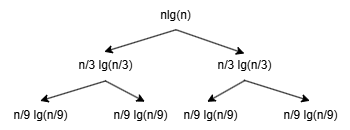
\includegraphics[width=.5\textwidth]{img/recurrence_tree_1.png}
    \label{fig:recurrence_tree_1}
\end{figure}

\noindent
Notiamo che il livello i-esimo dell'albero presenta un costo di $\left(\frac{2}{3}\right)^i n \lg \left(\frac{n}{3^i}\right)$. Con buona approssimazione possiamo ipotizzare che l'albero abbia profondita massima $\log_3 n$, dove vi sono $2^{log_{3}n}$ foglie, il cui costo è T(1). Quindi, il costo totale dell'ultimo livello è $T(1)\cdot 2^{\log_{3}{n}} = T(1)\cdot n^{log_{3}{2}} = \Theta(n^{log_{3} {2}})$.


\begin{equation} \label{eq:proof_1_4_1_1}
\begin{aligned}
T(n) & = \sum_{i=0}^{log_{3}{n} -1 } \left(\frac{2}{3}\right)^i n \lg{\frac{n}{3^i}} + \Theta(n^{log_{3}{2}}) \\
& = n \lg{n} \sum_{i=0}^{log_{3}{n} -1 }\left(\frac{2}{3}\right)^i - n \lg{n} \sum_{i=0}^{log_{3}{n} -1 }\left(\frac{2}{3}\right)^i \lg{3^i} + \Theta(n^{log_{3}{2}}) \\
& = n \lg{n} \sum_{i=0}^{log_{3}{n} -1 }\left(\frac{2}{3}\right)^i - n \lg{n} \sum_{i=0}^{log_{3}{n} -1 }i\left(\frac{2}{3}\right)^i \lg{3} + \Theta(n^{log_{3}{2}}) \\
& \le n \lg{n} \sum_{i=0}^{\infty}\left(\frac{2}{3}\right)^i + \Theta(n^{log_{3}{2}}) \\
& \le 3 n \lg{n}  + \Theta(n^{log_{3}{2}})
\end{aligned}
\end{equation}

\noindent Per questo motivo è possibile ipotizzare $T(n) = O(n\lg{n})$. Osservando poi che la prima chiamata costa proprio $n \lg{n}$, possiamo restringere l'ipotesi a $T(n) = \Theta(n \lg{n})$. L'ipotesi può essere verificata mediante il terzo caso del teorema dell'esperto:

\begin{equation} \label{eq:proof_1_4_1_2}
\begin{aligned}
n \lg{n} = \Omega(n^{\log_{3}{2} + \epsilon}); \ \text{se scegliamo } \epsilon = 0.27, \text{la condizione risulta verificata}.
\end{aligned}
\end{equation}

\begin{equation} \label{eq:proof_1_4_1_3}
\begin{aligned}
2 \frac{n}{3} \lg{\frac{n}{3}} &\le c n \lg{n} \\
\frac{2}{3} n \lg{n} - \frac{2}{3} n \lg{3} &\le c n \lg{n} \\
\left(\frac{2}{3} - c\right) \lg{n} &\le \frac{2}{3} \lg{3} \\
\end{aligned}
\end{equation}

\noindent  Tramite (\ref{eq:proof_1_4_1_2}) abbiamo verificato la prima ipotesi, mentre tramite (\ref{eq:proof_1_4_1_3}) verifichiamo la seconda scegliendo come costante $ 0 < c=\frac{2}{3} < 1$ per $n$ sufficientemente grande. Verificate le due ipotesi del terzo caso del teorema dell'esperto, possiamo concludere che l'ipotesi era corretta, ovvero $T(n) = \Theta(n lg{n})$.

\vspace{\baselineskip}

\noindent Per quanto riguarda la ricorrenza $T(n) = 3T(\frac{n}{5}) + \lg^2 n$, possiamo utilizzare il teorema dell'esperto per stabilire una forma chiusa per $T(n)$.


\begin{equation} \label{eq:proof_1_4_2_1}
\begin{aligned}
\lim_{n\to\infty} \frac{lg^k n}{n^\alpha} \text{, per } \ x = lg{x} \rightarrow \lim_{x\to\infty} \frac{x^k}{2^{\alpha k}} = 0 \quad \forall \alpha>0, \; \forall k>0.
\end{aligned}
\end{equation}

\noindent Per quanto stabilito in \ref{eq:proof_1_4_2_1}, possiamo affermare che $\lg^k n = O(n^\alpha)  \forall n>n_0 \ \text{e} \ \forall \alpha > 0, k>0$. Nel nostro caso $\lg^2 n = O(n^\alpha) \  \forall \alpha > 0$. Poichè $log_{5}{3} \approx 0.68 $, rientriamo nel primo caso del teorema dell'esperto, le cui ipotesi sono verificate in (\ref{eq:proof_1_4_2_2}).

\begin{equation} \label{eq:proof_1_4_2_2}
\begin{aligned}
\lg^2 n = O(n^{0.68 - \epsilon}) \; \text{scegliendo ad esempio } \; \epsilon = 0.1 > 0 \rightarrow \lg^2 n = O(n^{0.58})
\end{aligned}
\end{equation}

\noindent La (\ref{eq:proof_1_4_2_2}) risulta verificata per quanto asserito in (\ref{eq:proof_1_4_2_1}). In conclusione, per il teorema dell'esperto risulta $T(n) = \Theta(n^{\log_{5}{3}})$.


\subsection{Problema 1.1} \label{subsec:problema_1_1}
\textbf{Traccia}:

\noindent
\textit{Si implementi un algoritmo di ordinamento che sfrutta l'inserimento e la visita in un albero  binario di ricerca. Dato un vettore di n numeri interi in input, l'algoritmo procede prima ad 
inserire i numeri in un albero binario di ricerca (usando ripetutamente TREE-INSERT per inserire i numeri uno alla volta), e poi stampa i numeri in ordine con un attraversamento in ordine simmetrico dell'albero. Si analizzi la complessità nel caso peggiore e nel caso migliore per questo algoritmo di ordinamento.}

\vspace{2\baselineskip}
\noindent
\textbf{Soluzione}: 

\noindent
La soluzione presentata di seguito, così come gli altri problemi, è pensata in linguaggio c. Il file sorgente editabile \textit{"problem1\_1.c"} richiesto dalla consegna è presente nella directory \textit{problems} presente nel corrente archivio. Nel file sorgente sono presenti anche le implementazioni delle procedure di cui qui espongo solo la firma e le strutture dati utilizzate.

\begin{lstlisting}
#include <stdio.h>
#include <stdlib.h>

void tree_insert(Tree*, Node *);
void tree_init(Tree*);
void in_order_tree_walk(Node *);
void delete_tree(Tree *);

int main(int argc, char ** argv){
    int n = atoi(argv[1]);
    Tree * tree = (Tree*)malloc(sizeof(Tree));
    tree_init(tree);

    for(int i=0; i<n; i++){
        Node * new_node = (Node*)malloc(sizeof(Node));
        new_node->key=atoi(argv[i+2]);
        new_node->left = NULL;
        new_node->right = NULL;
        tree_insert(tree, new_node);
    }
    in_order_tree_walk(tree->root);
    delete_tree(tree);
    free(tree);
    return 0;
}

\end{lstlisting}
\noindent
L'input viene passato tramite linea di comando, e consiste in un intero che indica la dimensione dell'array da ordinare, seguito dagli interi costituenti l'array.

% Command-line "screenshot"
\begin{commandline}
\begin{verbatim}
$ gcc problem1_1.c -o problem1_1.exe
$ ./problem1_1.exe 7 1 2 3 4 5 6 7
1 2 3 4 5 6 7

$ ./problem1_1.exe 7 12 4 3 0 1 2 45 
0 1 2 3 4 12 45

$ ./problem1_1.exe 1 2 
2 

$ ./problem1_1.exe 0

$ ./problem1_1.exe 10 -1 -22 40 515 23 21 34 -541 99 0
-541 -22 -1 0 21 23 34 40 99 515
\end{verbatim}
\end{commandline}

\noindent
La complessità del ciclo for (linee 14-20) è determinata da n esecuzioni di tree\_insert, che ha complessità O(h) dove h è l'altezza dell'albero. La complessità $T(n) = O(nh)$. Nel caso migliore, l'albero è bilanciato quindi $h = \lg n$, e la complessità risulta $T(n) = O(n\lg n)$. Nel caso peggiore, l'input è costituito da dati già ordinati (caso di test 1) e questo comporta un'albero la cui altezza è $h = n$, e la complessità risulta $T(n) = O(n^2)$.
La procedura in\_order\_tree\_walk ha complessità O(n) poichè visita tutti i nodi una sola volta, quindi la complessità totale è dominata dal ciclo for (linee 14-20).

\subsection{Problema 1.2} \label{subsec:problema_1_2}
\textbf{Traccia}:

\noindent
\textit{Si implementi un algoritmo che, a partire da un vettore di n numeri interi in input, costruisce un heap chiamando ripetutamente la procedura MAX-HEAP-INSERT (vedi slide su 
heapsort) per inserire gli elementi nell'heap. L'algoritmo di costruzione ha il seguente 
pseudocodice:}

\begin{center}
	\begin{minipage}{0.5\linewidth} % Adjust the minipage width to accomodate for the length of algorithm lines
		\begin{algorithm}[H]
			\KwIn{$A$, array di n numeri interi}  % Algorithm inputs
			\medskip

            A.heap\_size = 1 \;
            \For{$i=2$ to A.lenght}{
                MAX\_HEAP\_INSERT(A, A[i])
            }
			\caption{\texttt{build\_max\_heap\_v2}} % Algorithm name
			\label{alg:max_heap_v2}   % optional label to refer to
		\end{algorithm}
	\end{minipage}
\end{center}


\noindent \textit{Si confronti la BUILD-MAX-HEAP vista a lezione con la BUILD-MAX-HEAP\_v2, in particolare: le due procedure creano sempre lo stesso heap se vengono eseguite con lo 
stesso array di input? Dimostrare che lo fanno o fornite un controesempio. Dimostrare che, nel caso peggiore, BUILD-MAX-HEAP\_v2 richiedo un tempo $\Theta(nlogn)$ per costruire un heap di n elementi. }

\vspace{2\baselineskip}
\noindent
\textbf{Soluzione}: 

\noindent
La soluzione presentata di seguito, così come gli altri problemi, è pensata in linguaggio c. Il file sorgente editabile \textit{"problem1\_2.c"} richiesto dalla consegna è presente nella directory \textit{problems} presente nel corrente archivio. Nel file sorgente sono presenti anche le implementazioni delle procedure di cui qui espongo solo la firma e le strutture dati utilizzate.

\begin{lstlisting}
#include <stdio.h>
#include <stdlib.h>
#define INF 50000

Heap* create_heap(int);
void swap(int*, int*);
void heap_increase_key(Heap*, int, int);
int parent(int);
void max_heap_insert(Heap*, int);
void build_max_heap_v2(Heap*, int*);
void print_heap(Heap*);
void delete_heap(Heap*);

int main(int argc, char** argv){
    int n = atoi(argv[1]);
    int input [n];
    Heap * h = create_heap(n);
    for(int i=0; i<n; i++){
        input[i]= atoi(argv[i+2]);
    }
    build_max_heap_v2(h, input);
    print_heap(h);
    delete_heap(h);
    free(h);
    return 0;
}


\end{lstlisting}
\noindent
L'input viene passato tramite linea di comando, e consiste in un intero che indica la dimensione dell'array con cui costruire l'heap, seguito dagli interi costituenti l'array. 



% Command-line "screenshot"
\begin{commandline}
\begin{verbatim}
$ gcc problem1_2.c -o problem1_2.exe
$ ./problem1_2.exe 5 4 2 3 5 1 
5 4 2 3 1

$ ./problem1_2.exe 6 12 1 6 9 3 
12 9 6 1 3 0 

$ ./problem1_2.exe 1 3 
3

$ ./problem1_2.exe 0

$ ./problem1_2.exe 6 12 1 6 9 3 1000
1000 9 12 1 3 6

$ ./problem1_2.exe 7 1 6 4 5 3 4 10
10 5 6 1 3 4 4

\end{verbatim}
\end{commandline}

\noindent
La procedura fin qui presentata garantisce che venga costruito un heap che rispetti le proprietà del max heap, così come la procedura vista a lezione. Tuttavia l'heap costruito potrebbe non essere uguale. Ad esempio, l'input \textit{<12 1 6 9 3 1000>} produce in output lo stesso heap \textit{<1000 9 12 1 3 6>}. Invece se l'input contiene numeri interi ripetuti, come nel caso di \textit{<7 1 6 4 5 3 4 10>}, l'output di BUILD-MAX-HEAP visto a lezione produce l'heap \textit{<10 6 1 5 3 4 4>} mentre BUILD-MAX-HEAP-v2 produce l'heap \textit{<10 5 6 1 3 4 4>}.

\noindent
Per quanto riguarda la complessità, questa risulta dominata dalla procedura build\_max\_heap\_v2. In questa procedura viene invocato n volte heap\_increase\_key, che ha complessità $O(log k)$, dove k sono gli elementi correntemente inseriti nell'heap. Sia T(n) la complessità associata alla procedura build\_max\_heap\_v2. 


\begin{equation} \label{eq:problem1_2}
\begin{aligned}
T(n) = \sum_{k=1}^{n} O(\lg(k))
\end{aligned}
\end{equation}

\noindent
Applicando la formula di Stirling $\lg{n!} \approx n \lg{n} - n = \Theta(n\lg{n})$, possiamo concludere che la complessità della procedura dominante è $\Theta(n\lg{n})$.



\subsection{Problema 1.3} \label{subsec:problema_1_3}
\textbf{Traccia}:

\noindent
\textit{Sia A[1 . . n] un array di n elementi distinti “quasi ordinato”, ovvero in cui ogni elemento dell'array si trova entro k slot dalla sua posizione corretta. Definiamo una "\textbf{inversione}": se i<j e A[i] > A[j], allora la coppia (i,j) è detta inversione di A. Si implementi un algoritmo che ordina il vettore A in tempo (n lg k). Suggerimento: Si usi un Heap.}

\vspace{2\baselineskip}
\noindent
\textbf{Soluzione}: 

\noindent
La soluzione presentata di seguito, così come gli altri problemi, è pensata in linguaggio c. Il file sorgente editabile \textit{"problem1\_3.c"} richiesto dalla consegna è presente nella directory \textit{problems} presente nel corrente archivio. Nel file sorgente sono presenti anche le implementazioni delle procedure di cui qui espongo solo la firma e le strutture dati utilizzate.

\newpage
\begin{lstlisting}
#include <stdio.h>
#include <stdlib.h>
#define INF 50000

void swap(int*, int*);
Heap * create_heap(int);
void destroy_heap(Heap*);
int left(int);
int right(int);
int parent(int);
void min_heapify(Heap *, int);
int extract_min(Heap *);
void heap_decrease_key(Heap*, int, int);
void min_heap_insert(Heap*, int);
void ordina(int *, int, int);

int main(int argc, char ** argv){
    int n = atoi(argv[1]);
    int k = atoi(argv[2]);
    int * input = (int*)malloc(n*sizeof(int)); 
    for(int i=0; i<n; i++) input[i] = atoi(argv[i+3]);
    ordina(input, n, k);
    for(int i=0; i<n; i++) printf("%d ", input[i]);
    printf("\n");
    free(input);
    return 0;
}



\end{lstlisting}
\noindent
L'input viene passato tramite linea di comando, e consiste in un intero che indica la dimensione dell'array da ordinare, un intero che indica le k posizioni entro cui si può trovare l'inversione, seguito dagli interi costituenti l'array. 



% Command-line "screenshot"
\begin{commandline}
\begin{verbatim}
$ gcc problem1_3.c -o problem1_3.exe
$ ./problem1_3.exe 5 4 2 3 5 1 
5 4 2 3 1

$ ./problem1_3.exe 7 3 6 5 3 2 8 10 9 
2 3 5 6 8 9 10

$ ./problem1_3.exe 11 3 1 2 4 5 6 3 9 11 12 13 10 
1 2 3 4 5 6 7 8 9 10

$ ./problem1_3.exe 0 9

$ ./problem1_3.exe 10 9 10 9 2 4 5 6 3 8 7 11
2 3 4 5 6 7 8 9 10 11
\end{verbatim}
\end{commandline}

\noindent
La complessità è determinata dalla procedura \textit{ordina()} che chiama n volte \textit{min\_heap\_insert()} su un heap di dimensione massima k ($O(\lg{k})$). La complessità è dunque $T(n) = \Theta(n\lg{k})$.



\newpage
\section{Homework set 2} \label{sec:homework_2}% Numbered section 


\subsection{Problema 2.1} \label{subsec:problema_2_1}
\textbf{Traccia}:

\noindent
\textit{Si consideri una matrice di 0 ed 1, in cui “1” indica “posizione occupata” e “0” indica “posizione libera”. Si scriva un algoritmo per determinare la sottomatrice massima libera (ossia che contiene tutti 0). L'algoritmo deve riportare il numero di 0 di tale sottomatrice.
Si alleghi al PDF un file editabile riportante l'implementazione in un linguaggio a scelta, corredato da almeno due casi di test con il corrispondente output atteso. Si forniscano i tre casi di test nello stesso formato del “sample input”. Si riporti la complessità.
}

\vspace{2\baselineskip}
\noindent
\textbf{Soluzione}: 

\noindent
La soluzione presentata di seguito, così come gli altri problemi, è pensata in linguaggio c. Il file sorgente editabile \textit{"problem2\_1.c"} richiesto dalla consegna è presente nella directory \textit{problems} presente nel corrente archivio. Nel file sorgente sono presenti anche le implementazioni delle procedure di cui qui espongo solo la firma e le strutture dati utilizzate.

\begin{lstlisting}
typedef struct {
    int top;
    int data[MAX];
} Stack;

void init_stack(Stack *);
int is_empty(Stack *);
void push(Stack*, int);
int pop(Stack*);
int top(Stack*);
int largest_rectangle(int*, int);
int max(int, int);


int main(){
    int i,j,N,M;
    int max_area = 0;

    // inizializza la matrice
    scanf("%d %d", &N, &M);
    int matrix[M][N];
    int hist[M];
    for(i=0; i<N; i++){
        for(j=0; j<M; j++){
            scanf("%d", &matrix[i][j]);
        }
    }

    memset(hist, 0, M*sizeof(int));
    for(i=0; i<N; i++){
        for(j=0; j<M; j++){
            if(matrix[i][j] == 0) hist[j] += 1;
            else hist[j] = 0;
        }

        max_area = max(max_area, largest_rectangle(hist, M));
    }

    printf("MAX AREA: %d\n", max_area);
}



\end{lstlisting}
\noindent
L'input  consiste in due interi che indicano le dimensioni della matrice, seguiti dagli interi rappresentanti i valori effettivi della matrice. L'output consiste nella dimensione della sottomatrice con più zeri contigui. 

% Command-line "screenshot"
\begin{commandline}
\begin{verbatim}
$ gcc problem2_1.c -o problem2_1.exe
$ ./problem2_1.exe 
6 4 
0 1 1 0
1 0 0 1
1 0 0 1
1 0 0 0
1 1 0 0 
0 1 0 1
MAX AREA: 6

$ ./problem2_1.exe 
4 4 
0 0 0 0
0 0 0 0
0 0 0 0
0 0 0 0
MAX AREA: 16

$ ./problem2_1.exe
4 4 
1 1 1 1 
1 1 1 1 
1 1 1 1 
1 1 1 1
MAX AREA: 0
\end{verbatim}
\end{commandline}

\noindent
Il main chiama N volte la procedura largest\_rectangle(). Questa procedura ha complessità $\Theta(M)$. La complessità totale è dunque $T(n) = \Theta(NM)$.


\subsection{Problema 2.2} \label{subsec:problema_2_2}
\textbf{Traccia}:

\noindent
\textit{Dato un array arr[] di dimensione n numeri interi, si scriva un algoritmo per trovare la lunghezza della sottosequenza crescente più lunga, ovvero la sottosequenza più lunga possibile in cui gli elementi sono ordinati in senso crescente. N.B una sottosequenza (diversamente da una sottostringa) può includere elementi non adiacenti.}

\noindent\textit{Si alleghi al PDF un file editabile riportante l'implementazione in un linguaggio a scelta, corredato da almeno due casi di test con il corrispondente output atteso. Si forniscano i tre casi di test nello stesso formato del “sample input”. Si riporti la complessità.}

\vspace{2\baselineskip}
\noindent
\textbf{Soluzione}: 

\noindent
La soluzione presentata di seguito, così come gli altri problemi, è pensata in linguaggio c. Il file sorgente editabile \textit{"problem2\_2.c"} richiesto dalla consegna è presente nella directory \textit{problems} presente nel corrente archivio. Nel file sorgente sono presenti anche le implementazioni delle procedure di cui qui espongo solo la firma e le strutture dati utilizzate.

\newpage
\begin{lstlisting}
int lis(int*, int);

int main(){
    int n,len;
    scanf("%d", &n);
    int arr[n];
    
    for(int i=0; i<n; i++){
        scanf("%d", &arr[i]);
    }
    len = lis(arr, n);
    printf("%d", len);
    return 0;
}

int lis(int* arr, int n){
    int dp[n];
    int len = 0;
    for(int i=0; i<n; i++) dp[i] = 1;

    for(int i=0; i<n; i++){
        for(int j=0; j<i; j++){
            if(arr[j] < arr[i]) dp[i] = max(dp[j]+1, dp[i]); 
        }
    }
}



\end{lstlisting}
\noindent
L'input consiste in un intero che indica la dimensione dell'array, seguito dagli interi rappresentanti i valori effettivi dell'array. L'output consiste nella dimensione della più lunga sottosequenza cresente. 

% Command-line "screenshot"
\begin{commandline}
\begin{verbatim}
$ gcc problem2_1.c -o problem2_1.exe
$ ./problem2_2.exe 
5
1 2 3 4 5
5

$ ./problem2_2.exe 
8
10 22 9 33 21 50 41 60
5

$ ./problem2_2.exe
6
6 5 4 3 2 1
1
\end{verbatim}
\end{commandline}

\noindent
La complessità è determinata dalla procedura lis(). In questa procedura, viene compilata la tabella degli stati dp[] tramite $n^2$ confronti, e ciò determina la complessità totale della procedura: $T(n) = \Theta(n^2)$.

\end{document}
% % Math equation/formula
% % \begin{equation}
% % 	I = \int_{a}^{b} f(x) \; \text{d}x.
% % \end{equation}

% % \begin{info} % Information block

% % \end{info}



% %------------------------------------------------


% % Numbered question, with subquestions in an enumerate environment
% % \begin{question}
% % 	Quisque ullamcorper placerat ipsum. Cras nibh. Morbi vel justo vitae lacus tincidunt ultrices. Lorem ipsum dolor sit amet, consectetuer adipiscing elit.

% % 	% Subquestions numbered with letters
% % 	\begin{enumerate}[(a)]
% % 		\item Do this.
% % 		\item Do that.
% % 		\item Do something else.
% % 	\end{enumerate}
% % \end{question}
	
% %------------------------------------------------

% \begin{center}
% 	\begin{minipage}{0.5\linewidth} % Adjust the minipage width to accomodate for the length of algorithm lines
% 		\begin{algorithm}[H]
% 			\KwIn{$(a, b)$, two floating-point numbers}  % Algorithm inputs
% 			\KwResult{$(c, d)$, such that $a+b = c + d$} % Algorithm outputs/results
% 			\medskip
% 			\If{$\vert b\vert > \vert a\vert$}{
% 				exchange $a$ and $b$ \;
% 			}
% 			$c \leftarrow a + b$ \;
% 			$z \leftarrow c - a$ \;
% 			$d \leftarrow b - z$ \;
% 			{\bf return} $(c,d)$ \;
% 			\caption{\texttt{FastTwoSum}} % Algorithm name
% 			\label{alg:fastTwoSum}   % optional label to refer to
% 		\end{algorithm}
% 	\end{minipage}
% \end{center}

% % % Numbered question, with an optional title
% % \begin{question}[\itshape (with optional title)]

% % \end{question}

% mappa della memoria 
% \begin{center}
    
%     \begin{tikzpicture}[scale=0.9]
%         % Rettangolo principale
%         \draw (0,0) rectangle (5,20);
%         \node at (2.4,20.3) {\textbf{Mappa memoria}};
        
%         % vuoto
%         \draw (0,20) rectangle (5,19);
%         \node[right=5pt] at (5,19.5) {\texttt{\$00000000}};
%         \fill[lightgray] (0,20) rectangle (5,19);
%         % INT3
%         \fill[red!20](0,19) rectangle (5,17);
%         \draw (0,19) rectangle (5,18);
%         \node[left=5pt] at (0,18.5) {ISR\_B};
%         \node[right=5pt] at (5,18.5) {\texttt{\$0000006C}};
%         \node at (2.5,18.5) {\$00008700}; 
        
%         % INT4 
%         \draw (0,18) rectangle (5,17);
%         \node[left=5pt] at (0,17.5) {ISR\_C};
%         \node[right=5pt] at (5,17.5) {\texttt{\$00000070}};
%         \node at (2.5,17.5) {\$00008800};

%         % vuoto
%         \draw (0,17) rectangle (5,16);
%         \fill[lightgray] (0,17) rectangle (5,16);
%         %PIA 
%         \fill[yellow!20](0,16) rectangle (5,8);
%         \draw(0,16) rectangle (5,15);
%         \node[right=5pt] at (5,15.5) {\texttt{\$00002004}};
%         \node at (2.5,15.5) {PIABPRA};
%         \draw(0,15) rectangle (5,14);
%         \node[right=5pt] at (5,14.5) {\texttt{\$00002005}};
%         \node at (2.5,14.5) {PIABCRA};
%         \draw(0,14) rectangle (5,13);
%         \node[right=5pt] at (5,13.5) {\texttt{\$00002006}};
%         \node at (2.5,13.5) {PIABPRB};
%         \draw(0,13) rectangle (5,12);
%         \node[right=5pt] at (5,12.5) {\texttt{\$00002007}};
%         \node at (2.5,12.5) {PIABCRB};

%         \draw(0,12) rectangle (5,11);
%         \node[right=5pt] at (5,11.5) {\texttt{\$00002008}};
%         \node at (2.5,11.5) {PIACPRA};
%         \draw(0,11) rectangle (5,10);
%         \node[right=5pt] at (5,10.5) {\texttt{\$00002009}};
%         \node at (2.5,10.5) {PIACCRA};
%         \draw(0,10) rectangle (5,9);
%         \node[right=5pt] at (5,9.5) {\texttt{\$0000200A}};
%         \node at (2.5,9.5) {PIACPRB};
%         \draw(0,9) rectangle (5,8);
%         \node[right=5pt] at (5,8.5) {\texttt{\$0000200B}};
%         \node at (2.5,8.5) {PIACCRB};

%         % vuoto
%         \draw (0,8) rectangle (5,7);
%         \fill[lightgray] (0,8) rectangle (5,7);
        
%         % DATI
%         \fill[green!10] (0,7) rectangle (5,0);
%         \draw(0,7) rectangle (5,6);
%         \node[right=5pt] at (5,6.5) {\texttt{\$00008000}};
%         \node at (2.5,6.5) {AREA DATI};

        
%         % vuoto
%         \draw (0,6) rectangle (5,5);
%         \fill[lightgray] (0,6) rectangle (5,5);
        
%         % CODICE
%         \draw(0,5) rectangle (5,4);
%         \node[right=5pt] at (5,4.5) {\texttt{\$00008200}};
%         \node at (2.5,4.5) {AREA CODICE};

%         % vuoto
%         \draw (0,4) rectangle (5,3);
%         \fill[lightgray] (0,4) rectangle (5,3);

%         % ISRB 
%         \draw(0,3) rectangle (5,2);
%         \node[right=5pt] at (5,2.5) {\texttt{\$00008700}};
%         \node at (2.5,2.5) {ISR\_B};

%         % vuoto
%         \draw (0,2) rectangle (5,1);
%         \fill[lightgray] (0,2) rectangle (5,1);

%         % ISRC
%         \draw(0,1) rectangle (5,0);
%         \node[right=5pt] at (5,0.5) {\texttt{\$00008800}};
%         \node at (2.5,0.5) {ISR\_C};

%         % vuoto 
%         \draw(0,0) rectangle (5,-1);
%         \fill[lightgray](0,0) rectangle (5,-1);
%         % STACK
%         \fill[blue!20](0,-1) rectangle (5,-2);
%         \draw (0,-1) rectangle (5,-2);
%         \node[right=5pt] at (5,-1.5) {\texttt{\$00009000}};
%         \node at (2.5,-1.5) {STACK U-S};

%         \draw(0,-2) rectangle (5,20); % ricalco bordi
%     \end{tikzpicture}
% \end{center}

% % % File contents
% % \begin{file}[hello.py]
% % \begin{lstlisting}[language=Python]
% % #! /usr/bin/python

% % import sys
% % sys.stdout.write("Hello World!\n")
% % \end{lstlisting}
% % \end{file}



% % % Command-line "screenshot"
% % \begin{commandline}
% % 	\begin{verbatim}
% % 		$ chmod +x hello.py
% % 		$ ./hello.py

% % 		Hello World!
% % 	\end{verbatim}
% % \end{commandline}


% % Warning text, with a custom title
% % \begin{warn}[Osservazione:]

% % \end{warn}

% %----------------------------------------------------------------------------------------


% tabella in formato testuale molto cool ben indentata 
% \begin{description}[style=nextline,leftmargin=3.45cm,labelwidth=2.8cm,labelsep=0.6cm,font=\ttfamily\bfseries]
%   \item[fine] Intero che può assumere i valori 0 (il nodo A è in ricezione) o 1 (il nodo A ha terminato la ricezione).

% \end{description}

% \begin{lstlisting}
% c code snippet  
% \end{lstlisting}



% \begin{lstlisting}[language=RISCAsm]
% asm code snippet
% \end{lstlisting}


